\documentclass[aspectratio=169,xcolor=dvipsnames]{beamer}

%----------------------------------------------------------------------------------------
%    PACKAGES AND THEMES
%----------------------------------------------------------------------------------------

\usetheme{SimplePlus}
% Definizione di un ambiente personalizzato simile a "examples" ma con titolo variabile
\newenvironment{customexampleblock}[1]{%
  \setbeamercolor{block title}{bg=Green, fg=white} % Colore del titolo (come in 'examples')
  \setbeamercolor{block body}{bg=Green!10, fg=black} % Colore del corpo (un verde chiaro)
  \begin{block}{#1}
}{%
  \end{block}
}

\usepackage[utf8]{inputenc}
\usepackage[T1]{fontenc}
\usepackage[english]{babel}
\usepackage{amsmath, amssymb}
\usepackage{graphicx} % Allows including images
\usepackage{booktabs} % Allows the use of \toprule, \midrule and \bottomrule in tables
\usepackage{multirow}
\usepackage{hyperref}
\usepackage{fontspec}
% Carica il font delle emoji di Windows 11
\newfontface{\fluentemoji}{Segoe UI Emoji}[Renderer=HarfBuzz]

% Crea un comando per usare facilmente le emoji
\newcommand{\emoji}[1]{{\fluentemoji #1}}

% Crea un comando specifico per il razzo per comodità
\newcommand{\rocket}{\emoji{🚀}}

%----------------------------------------------------------------------------------------
%    TITLE PAGE
%----------------------------------------------------------------------------------------

\title{Toxicity, couple dynamics and most toxic sentence detection in Italian conversations using classical machine learning models and transformer-based models}
\subtitle{} % No subtitle in the original, left empty

\author{Davide Cirilli}

\institute
{
    Università degli Studi di Bari Aldo Moro
}
\date{} % Date left empty as in the original

%----------------------------------------------------------------------------------------
%    PRESENTATION SLIDES
%----------------------------------------------------------------------------------------

\begin{document}

\begin{frame}
    % Print the title page as the first slide
    \titlepage
\end{frame}

\begin{frame}{Overview}
    % The \tableofcontents command will automatically list your sections and subsections
    \tableofcontents
\end{frame}

%------------------------------------------------
\section{Introduction and Motivations}
%------------------------------------------------

\begin{frame}
\frametitle{Context and Goals}

\begin{block}{Why this work matters}
\begin{itemize}
\item Toxic behaviors in online conversations can cause serious psychological and social harm.
\item Italian conversational toxicity and personality-driven patterns are underexplored in NLP research.
\item There is a need for systems that go beyond keyword detection to capture complex interaction dynamics.
\end{itemize}
\end{block}

\begin{block}{Our contribution}
\begin{itemize}
\item A system combining toxicity detection and personality analysis in Italian dialogues.
\item Integration of classical ML (e.g., Logistic Regression, Naive Bayes) and transformer models (BERT, BART).
\item A web app for interactive real-time couple dynamics and toxic sentence detection.
\end{itemize}
\end{block}

\end{frame}

%------------------------------------------------
\section{Dataset}
%------------------------------------------------

\begin{frame}
\frametitle{Preprocessing and Generation Settings}

\begin{block}{Toxic data preprocessing}
\begin{itemize}
\item Removed incomplete / malformed entries
\item Extracted most toxic sentence via regular expressions
\item Normalized whitespace, punctuation, and symbols
\end{itemize}
\end{block}

\begin{customexampleblock}{Non-toxic data generation and parameters}
\begin{itemize}
\item \textbf{Model}: \textbf{gemini-2.0-flash-lite} via \textbf{API + Google AI Studio}
\item \textbf{Generation Settings}:
\begin{itemize}
\item \textbf{Temperature}: 1.8
\item \textbf{Top-p}: 1.0
\item \textbf{Top-k}: 0
\item \textbf{Safety filters}: BLOCK\_MEDIUM\_AND\_ABOVE (harassment, hate speech, explicit, dangerous)
\end{itemize}
\end{itemize}
\end{customexampleblock}

\end{frame}

\begin{frame}
\frametitle{Final Dataset Composition}

\begin{block}{Toxic Conversations}
\begin{itemize}
\item \textasciitilde 950 Italian dialogues with toxic dynamics
\item Includes manipulation, emotional control, psychological abuse
\item Annotated with relationship type and most toxic sentence
\end{itemize}
\end{block}

\begin{block}{Non-Toxic Conversations}
\begin{itemize}
\item \textasciitilde 600 synthetic dialogues created with Gemini API and Google AI Studio
\item Healthy, culturally appropriate interactions
\item 5 Positive dynamics: \textit{Supportive-Insecure}, \textit{Collaborative-Propositive}, etc.
\end{itemize}
\end{block}

\end{frame}

%------------------------------------------------
\section{Approach}
%------------------------------------------------

\subsection{Binary Toxic Classification}

\begin{frame}
\frametitle{Binary Toxic Classification: Overview}

\begin{block}{Goal}
Classify conversations as \textbf{toxic} or \textbf{non-toxic} based on dialogue content.
\end{block}

\begin{block}{Modeling strategies}
\begin{itemize}
\item Traditional ML with TF-IDF + Logistic Regression
\item Traditional ML with TF-IDF + Multinomial Naive Bayes
\item Experiments with and without linguistic preprocessing
\end{itemize}
\end{block}

\end{frame}

\begin{frame}
\frametitle{Binary Toxic Classification: Details}

\begin{block}{Preprocessing variants}
\begin{itemize}
\item \textbf{Without preprocessing:} raw text, tokenized, bi-gram TF-IDF
\item \textbf{With preprocessing:} spaCy Italian model (lemmatization, stopword and punctuation removal, lowercasing)
\end{itemize}
\end{block}

\begin{customexampleblock}{Training parameters}
\begin{itemize}
\item 80-20 stratified train/test split
\item Grid search + 5-fold stratified CV
\item TF-IDF bi-grams, max\_features tuned (2000-7000)
\item Logistic Regression: tuned $C \in \{0.1, 1, 10\}$
\item Naive Bayes: tuned $\alpha \in \{0.1, 1\}$
\end{itemize}
\end{customexampleblock}

\end{frame}

\subsection{Couple Dynamics Prediction}

\begin{frame}
\frametitle{Couple Dynamics Prediction: Task and Goal}

\begin{block}{Objective}
Classify the conversational dynamic between two participants into one of 15 predefined relationship types.
\end{block}

\begin{block}{Examples of classes}
\begin{itemize}
\item \textit{Narcissist and Submissive}
\item \textit{Manipulator and Emotionally Dependent}
\item \textit{Supportive and Insecure}
\item \textit{Grateful and Appreciative}
\end{itemize}
\end{block}

\end{frame}

\begin{frame}
\frametitle{Couple Dynamics Prediction: Modeling Approaches}

\begin{block}{Explored approaches}
\begin{itemize}
\item \textbf{TF-IDF + LSA + Logistic Regression}
\item \textbf{Frozen BERT embeddings + Logistic Regression}
\item \textbf{Fine-tuned BERT}
\end{itemize}
\end{block}

\begin{block}{Pipeline differences}
\begin{itemize}
\item LSA: dimensionality reduction with TruncatedSVD
\item Frozen BERT: [CLS] embeddings without task-specific tuning
\item Fine-tuned BERT: direct adaptation to the classification task
\end{itemize}
\end{block}

\vspace{0.3cm}
\begin{center}
\colorbox{blue!10}{\parbox{0.8\linewidth}{\centering BERT model: \texttt{dbmdz/bert-base-italian-uncased}}}
\end{center}

\end{frame}

\begin{frame}
\frametitle{Couple Dynamics Prediction: Training Configurations}

\begin{block}{TF-IDF + LSA + Logistic Regression}
\begin{itemize}
\item Unigrams and bigrams TF-IDF
\item SVD components: 100, 200, 300 (grid search)
\item Logistic Regression: $C \in \{0.1, 1, 10\}$ (lbfgs solver)
\end{itemize}
\end{block}

\begin{block}{Frozen BERT + Logistic Regression}
\begin{itemize}
\item Extract [CLS] token embeddings
\item Logistic Regression: $C = 0.1$, max 2000 iterations
\end{itemize}
\end{block}

\begin{customexampleblock}{Fine-tuned BERT}
\begin{itemize}
\item Adam + weight decay, learning rate warmup
\item Batch size: 8, max length: 512
\item Up to 7 epochs, early stopping (patience = 2)
\item Evaluation: accuracy, macro precision, recall, F1
\end{itemize}
\end{customexampleblock}

\end{frame}

\subsection{Most Toxic Sentence Detection}

\begin{frame}
\frametitle{Most Toxic Sentence Detection: Task and Goal}

\begin{block}{Objective}
Identify or generate the most toxic sentence within a given conversation.
\end{block}

\begin{block}{Challenges}
\begin{itemize}
\item Toxic phrases can be subtle, context-dependent, or implicit.
\item Class imbalance: toxic sentences are rare compared to non-toxic ones.
\item Open-ended phrasing makes exact match generation difficult.
\end{itemize}
\end{block}

\vspace{0.3cm}
\begin{center}
\colorbox{yellow!10}{\parbox{0.8\linewidth}{\centering Two complementary approaches: classification and generation}}
\end{center}

\end{frame}

\begin{frame}
\frametitle{Most Toxic Sentence Detection: Classification Approach}

\begin{block}{Model}
Fine-tuned BERT (\texttt{dbmdz/bert-base-italian-uncased})
\end{block}

\begin{block}{Pipeline}
\begin{itemize}
\item Input: individual message + couple dynamic type (as additional context)
\item Output: toxicity probability for each message
\item Most toxic sentence = message with highest toxicity probability
\end{itemize}
\end{block}

\begin{customexampleblock}{Training configuration}
\begin{itemize}
\item Max length: 128 tokens
\item Batch size: 32, learning rate: $2 \times 10^{-5}$
\item AdamW optimizer, weight decay: 0.01
\item Up to 7 epochs, early stopping (patience = 2)
\item Stratified 80/10/10 split: train/val/test
\end{itemize}
\end{customexampleblock}

\end{frame}

\begin{frame}
\frametitle{Most Toxic Sentence Detection: Generation Approach}

\begin{block}{Model}
Fine-tuned BART (\texttt{facebook/bart-base})
\end{block}

\begin{block}{Pipeline}
\begin{itemize}
\item Input: full conversation prefixed with a task descriptor
\item Output: generated most toxic sentence
\item Generation decoding: beam search (4 beams), early stopping
\end{itemize}
\end{block}

\begin{customexampleblock}{Training configuration}
\begin{itemize}
\item Max input length: 512 tokens, output: 64 tokens
\item Batch size: 4, learning rate: $3 \times 10^{-5}$
\item Early stopping (patience = 2)
\item GroupShuffleSplit to avoid similar conversations across sets
\end{itemize}
\end{customexampleblock}

\end{frame}

\subsection{Web Application}

\begin{frame}
\frametitle{Web Application: Summary}

\begin{block}{Purpose}
\begin{itemize}
\item Real-time couple dynamics classification
\item Most toxic sentence detection (classification + generation)
\end{itemize}
\end{block}

\begin{block}{Key features}
\begin{itemize}
\item Chat-like interface, dynamic updates after each input
\item On-demand toxic phrase extraction (classification + seq2seq)
\end{itemize}
\end{block}

\vspace{0.2cm}
\begin{center}
\colorbox{blue!10}{\parbox{0.8\linewidth}{\centering Built with Gradio}}
\end{center}

\end{frame}

%------------------------------------------------
\section{Results}
%------------------------------------------------

\subsection{Binary Toxicity Classification}

\begin{frame}
\frametitle{Binary Toxicity Classification: Performance Summary}

\begin{table}
\centering
\begin{tabular}{lcccc}
\toprule
\textbf{Model} & \textbf{Accuracy} & \textbf{Precision} & \textbf{Recall} & \textbf{F1} \\
\midrule
Logistic Regression (raw) & 0.9968 & 0.9968 & 0.9968 & 0.9968 \\
Naive Bayes (raw) & 0.9968 & 0.9968 & 0.9968 & 0.9968 \\
Logistic Regression (spaCy) & 0.9936 & 0.9936 & 0.9936 & 0.9936 \\
Naive Bayes (spaCy) & 0.9968 & 0.9968 & 0.9968 & 0.9968 \\
\bottomrule
\end{tabular}
\caption{Binary toxicity classification results}
\end{table}

\vspace{0.2cm}
\begin{center}
\colorbox{blue!10}{\parbox{0.7\linewidth}{\centering Near-perfect performance across all configurations}}
\end{center}

\end{frame}

\begin{frame}
\frametitle{Binary Toxicity Classification: Confusion Matrices (Raw Text)}

\begin{columns}[c]
\begin{column}{0.5\textwidth}
\begin{figure}
\centering
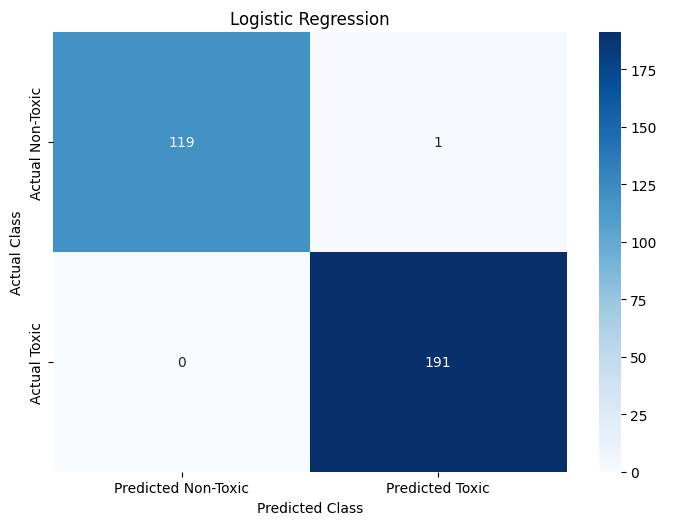
\includegraphics[width=\linewidth]{figures/confusion_lr_no_pre.png}
\caption{Logistic Regression (raw text)}
\end{figure}
\end{column}

\begin{column}{0.5\textwidth}
\begin{figure}
\centering
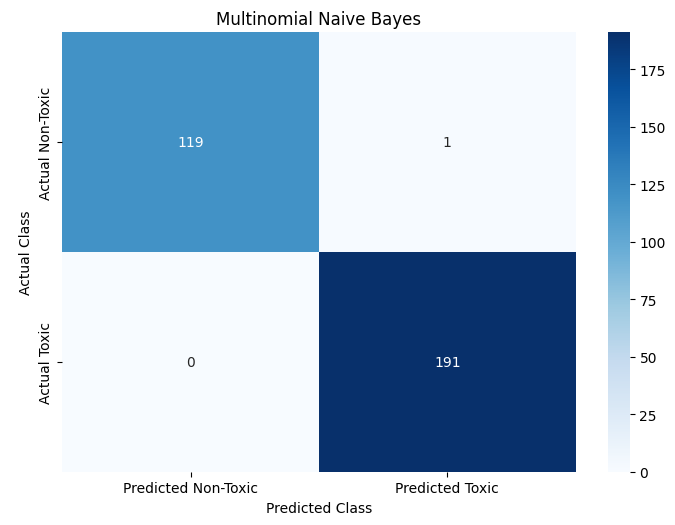
\includegraphics[width=\linewidth]{figures/confusion_nb_no_pre.png}
\caption{Naive Bayes (raw text)}
\end{figure}
\end{column}
\end{columns}

\end{frame}

\begin{frame}
\frametitle{Binary Toxicity Classification: Confusion Matrices (spaCy Processed)}

\begin{columns}[c]
\begin{column}{0.5\textwidth}
\begin{figure}
\centering
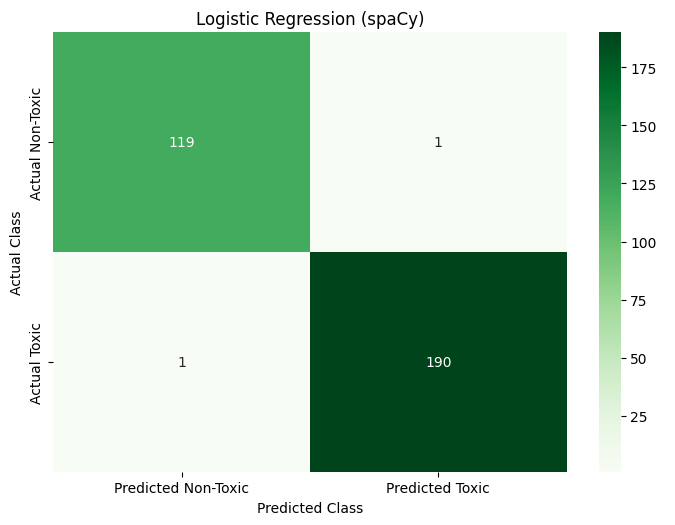
\includegraphics[width=\linewidth]{figures/confusion_lr_spacy.png}
\caption{Logistic Regression (spaCy processed)}
\end{figure}
\end{column}

\begin{column}{0.5\textwidth}
\begin{figure}
\centering
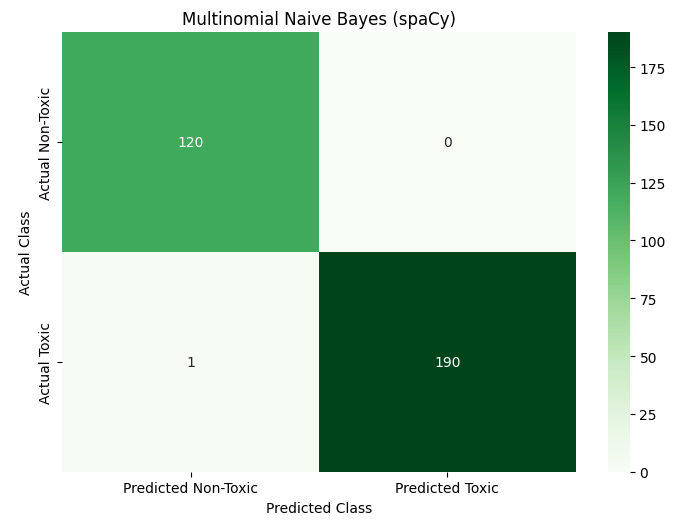
\includegraphics[width=\linewidth]{figures/confusion_nb_spacy.png}
\caption{Naive Bayes (spaCy processed)}
\end{figure}
\end{column}
\end{columns}

\end{frame}

\subsection{Couple Dynamics Prediction}

\begin{frame}
\frametitle{Couple Dynamics Prediction: Performance Summary}

\begin{table}
\centering
\begin{tabular}{lcccc}
\toprule
\textbf{Approach} & \textbf{Accuracy} & \textbf{Precision} & \textbf{Recall} & \textbf{F1} \\
\midrule
LSA + Logistic Regression & 0.7395 & 0.7233 & 0.7160 & 0.7113 \\
Frozen BERT + Logistic Regression & 0.7010 & 0.6840 & 0.6767 & 0.6753 \\
Fine-tuned BERT & 0.8013 & 0.8093 & 0.7867 & 0.7780 \\
\bottomrule
\end{tabular}
\caption{Couple dynamics classification results (macro average)}
\end{table}

\vspace{0.2cm}
\begin{center}
\colorbox{blue!10}{\parbox{0.75\linewidth}{\centering Fine-tuned BERT outperforms other approaches}}
\end{center}

\end{frame}

\begin{frame}
\frametitle{Couple Dynamics Prediction: Confusion Matrices}

\begin{columns}[c]
\column{0.5\textwidth}
    \begin{figure}
    \centering
    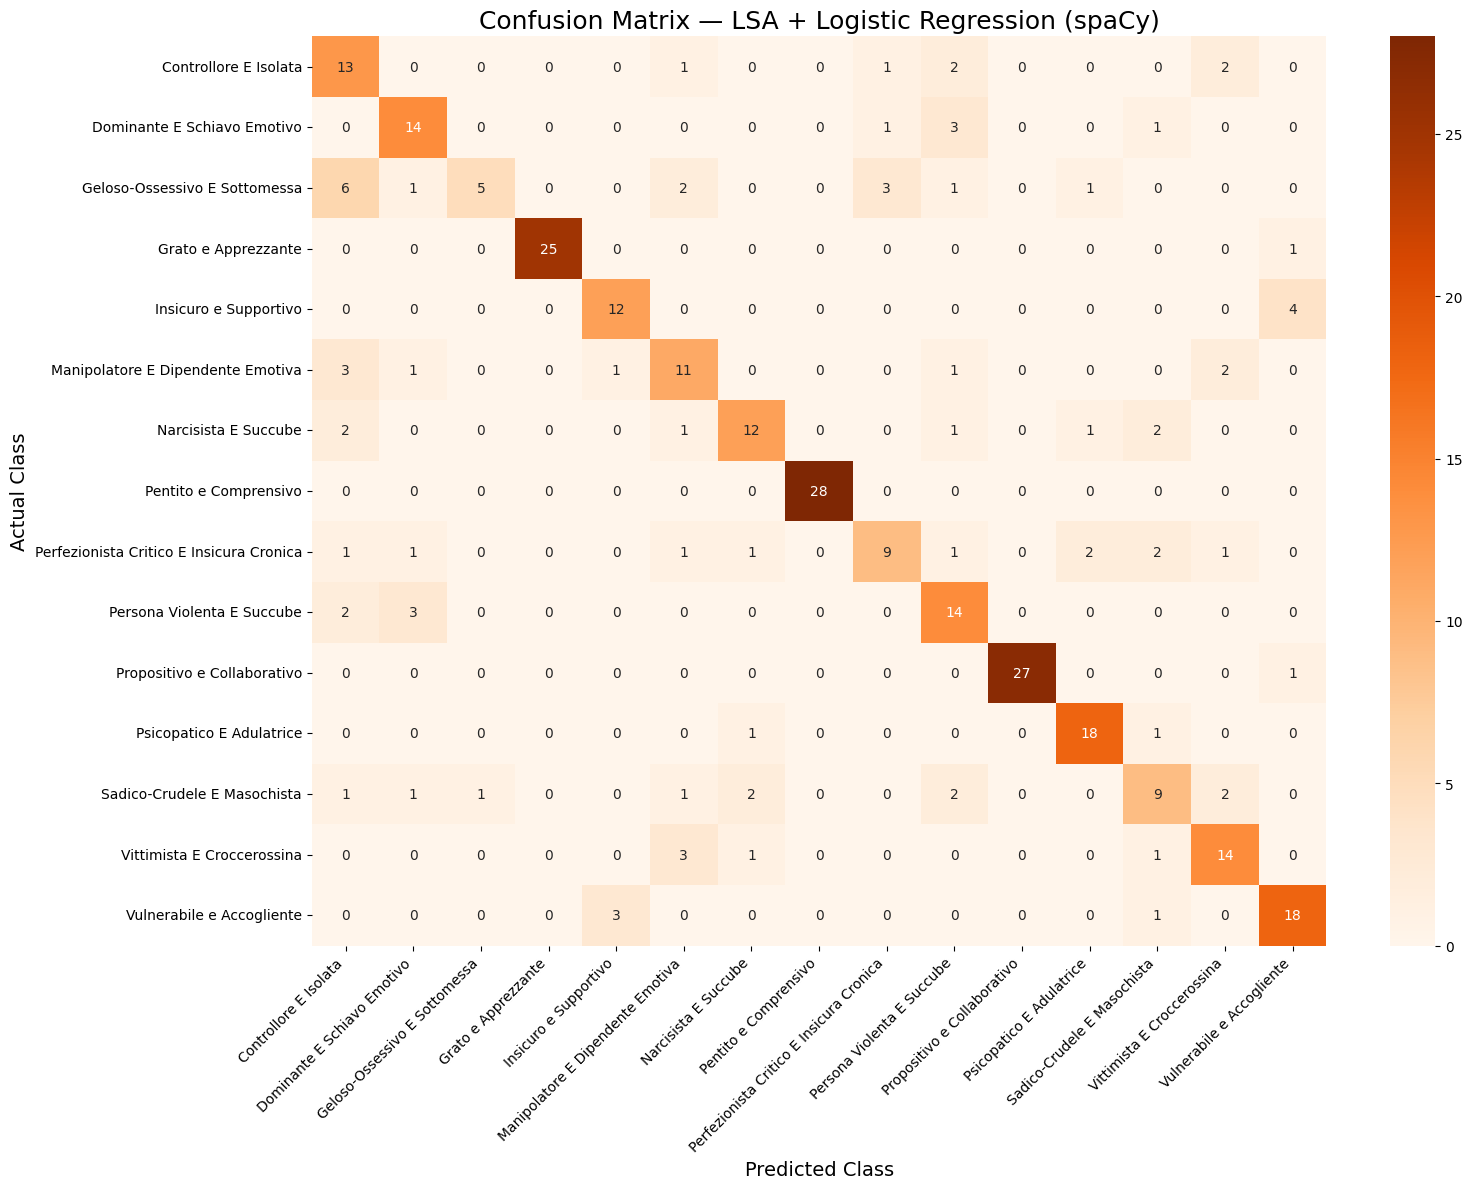
\includegraphics[width=\linewidth]{figures/lsa_logreg_confusion_matrix.png}
    \caption{Confusion matrix - LSA + Logistic Regression}
    \end{figure}
\column{0.5\textwidth}
    \begin{figure}
    \centering
    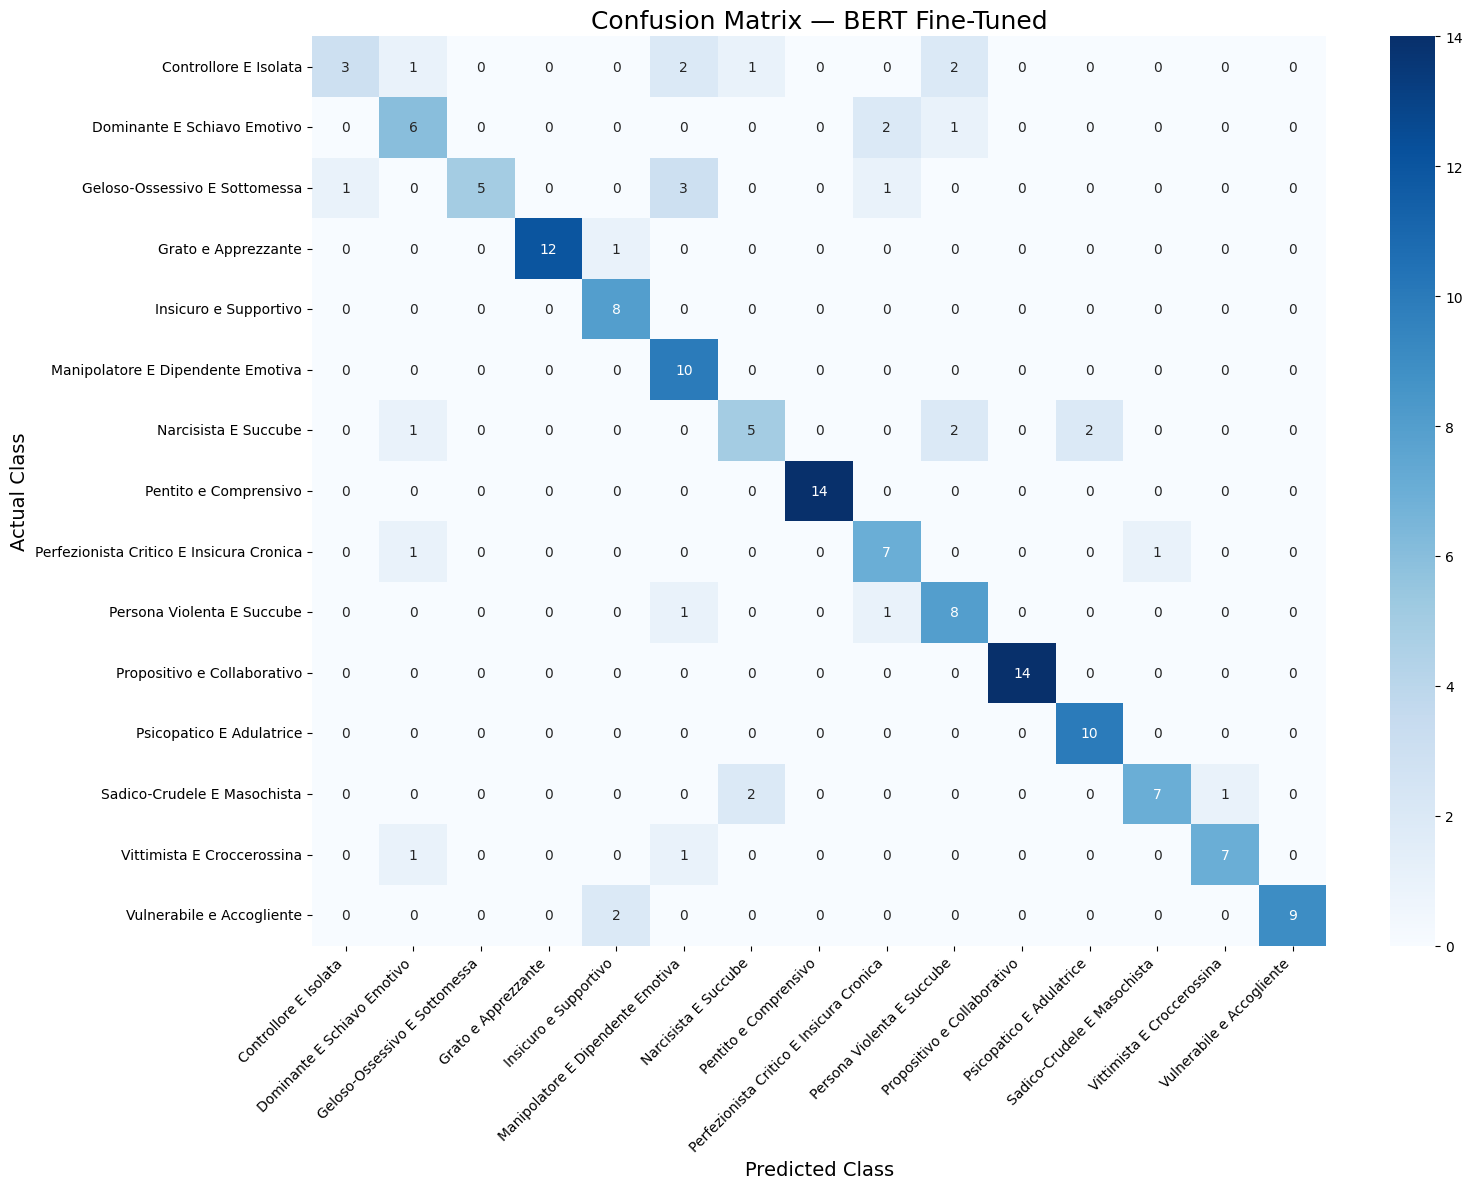
\includegraphics[width=\linewidth]{figures/bert_finetuned_confusion_matrix.png}
    \caption{Confusion matrix - Fine-tuned BERT}
    \end{figure}
\end{columns}

\end{frame}

\begin{frame}
\frametitle{Couple Dynamics Prediction: Fine-tuned BERT Loss Curves}

\begin{figure}
\centering
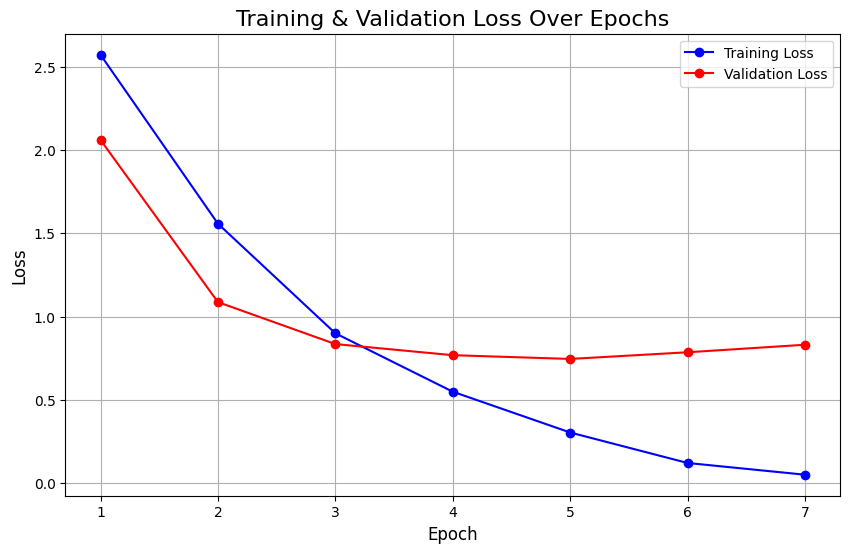
\includegraphics[width=0.6\linewidth]{figures/bert_finetuned_loss_curves.png}
\caption{Training and validation loss during fine-tuning}
\end{figure}

\vspace{0.1cm}
\begin{center}
\colorbox{green!10}{\parbox{0.8\linewidth}{\centering Good convergence with no significant overfitting observed}}
\end{center}

\end{frame}

\subsection{Most Toxic Sentence Detection}

\begin{frame}
\frametitle{Most Toxic Sentence Detection: Classification Results}

\begin{table}
\centering
\begin{tabular}{lcccc}
\toprule
\textbf{Class} & \textbf{Precision} & \textbf{Recall} & \textbf{F1-score} & \textbf{Support} \\
\midrule
Non-Toxic & 0.9077 & 0.9558 & 0.9311 & 679 \\
Toxic & 0.3617 & 0.2048 & 0.2615 & 83 \\
\midrule
Accuracy & \multicolumn{4}{c}{0.8740} \\
Macro avg & 0.6347 & 0.5803 & 0.5963 & 762 \\
Weighted avg & 0.8482 & 0.8740 & 0.8582 & 762 \\
\bottomrule
\end{tabular}
\caption{Performance of BERT toxic phrase classification (test set)}
\end{table}

\vspace{0.2cm}
\begin{center}
\colorbox{blue!10}{\parbox{0.75\linewidth}{\centering High accuracy but low recall on toxic class}}
\end{center}

\end{frame}

\begin{frame}
\frametitle{Most Toxic Sentence Detection: Confusion Matrix}

\begin{figure}
\centering
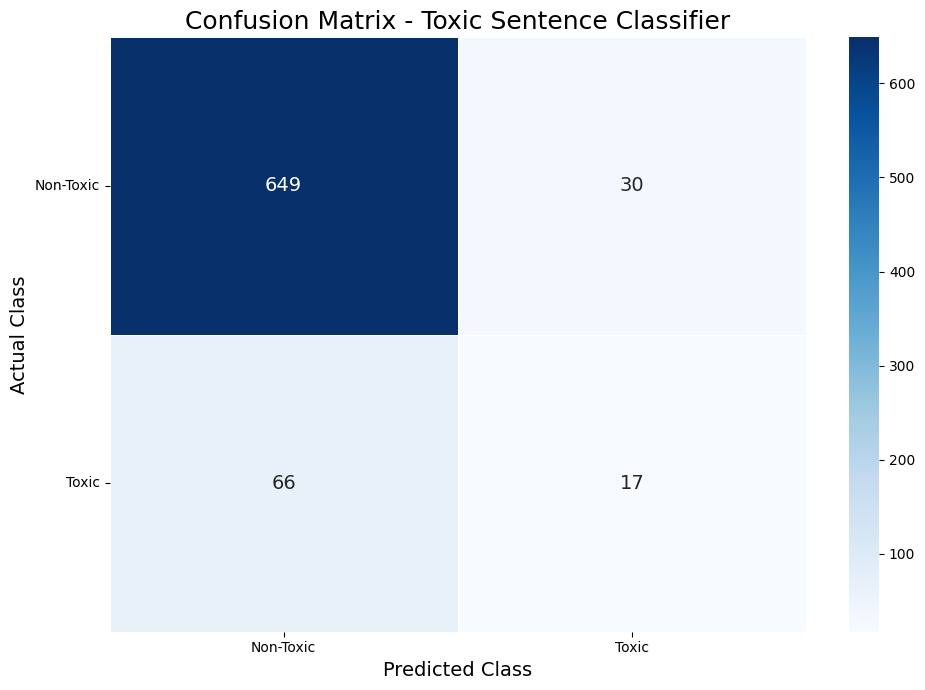
\includegraphics[width=0.6\linewidth]{figures/bert_toxic_confusion_matrix.png}
\caption{Confusion matrix - BERT classification model}
\end{figure}

\end{frame}

\begin{frame}
\frametitle{Most Toxic Sentence Generation: Results}

\begin{table}
\centering
\begin{tabular}{lc}
\toprule
\textbf{Metric} & \textbf{Score} \\
\midrule
BLEU & 0.1706 \\
ROUGE-1 F1 & 0.3031 \\
ROUGE-2 F1 & 0.2170 \\
ROUGE-L F1 & 0.2987 \\
\bottomrule
\end{tabular}
\caption{BART toxic phrase generation performance}
\end{table}

\vspace{0.2cm}
\begin{center}
\colorbox{green!10}{\parbox{0.8\linewidth}{\centering Captured some key n-grams, but generation remains challenging}}
\end{center}

\end{frame}

\begin{frame}
\frametitle{Most Toxic Sentence Generation: Loss Curves}

\begin{figure}
\centering
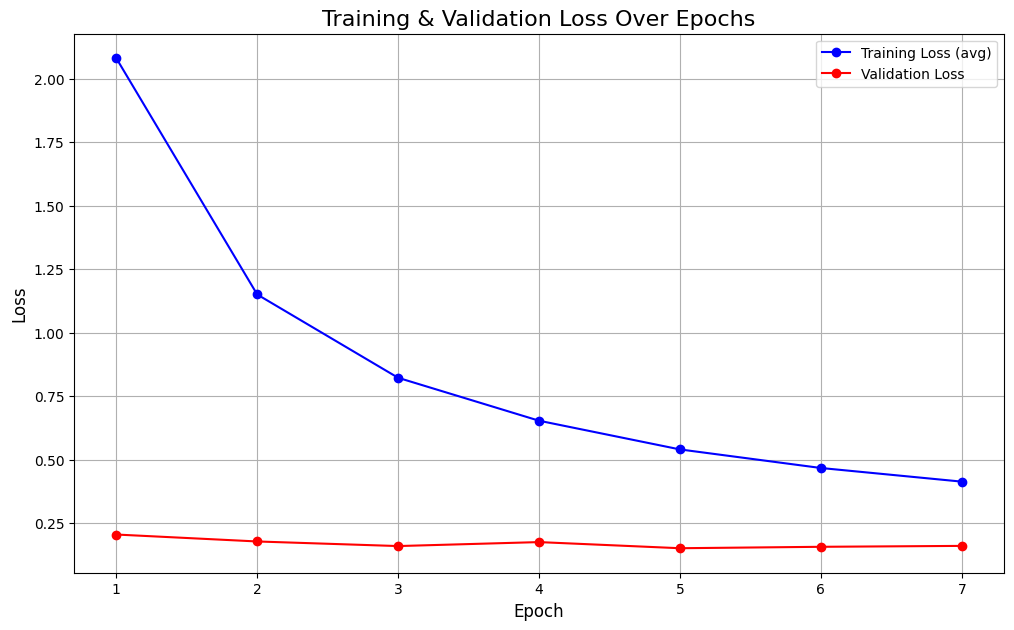
\includegraphics[width=0.6\linewidth]{figures/bart_toxic_loss_curves.png}
\caption{Training and validation loss - BART generation model}
\end{figure}

\vspace{0.1cm}
\begin{center}
\colorbox{yellow!10}{\parbox{0.75\linewidth}{\centering Stable validation loss; no major overfitting detected}}
\end{center}

\end{frame}

\subsection{Web Application}

\begin{frame}
\frametitle{Web Application Interface}

\begin{figure}
\centering
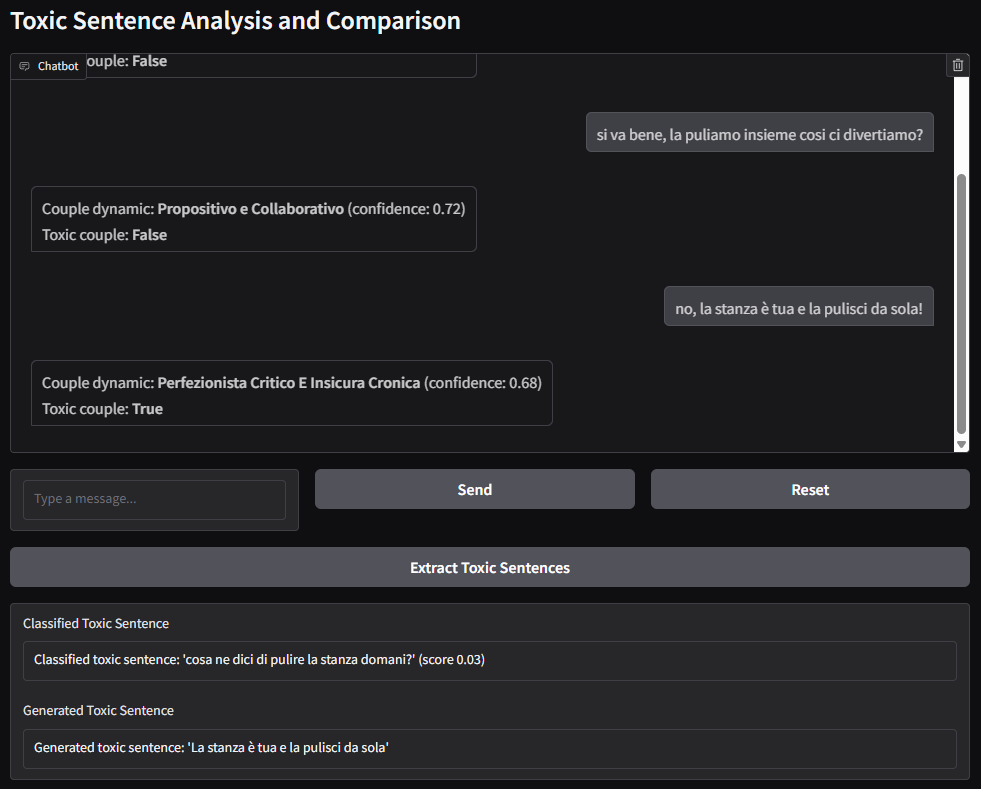
\includegraphics[width=0.55\linewidth]{figures/web_app_interface_used.png}
\caption{Screenshot of the interactive web interface}
\end{figure}

\end{frame}

%------------------------------------------------
\section{Conclusion}
%------------------------------------------------

\begin{frame}
\frametitle{Key Contributions and Results Summary}

\begin{block}{Key contributions}
\begin{itemize}
\item Created balanced dataset (\textasciitilde 1550 dialogues, annotated toxic phrases).
\item Combined toxicity detection and couple dynamics classification for Italian dialogues.
\item Integrated classical ML and transformer models for multi-task learning.
\item Developed interactive web app for real-time predictions.
\end{itemize}
\end{block}

\begin{block}{Results highlights}
\begin{itemize}
\item \textbf{Binary toxicity classification:} accuracy up to 99.7\%.
\item \textbf{Couple dynamics prediction:} fine-tuned BERT with 80\% accuracy.
\item \textbf{Toxic phrase detection:} high overall accuracy, challenges on minority class.
\item \textbf{Toxic phrase generation:} achieved moderate results, capturing key n-grams and contextual nuances.
\end{itemize}
\end{block}

\end{frame}

\begin{frame}
\frametitle{Current Limitations \& Future Directions}

\begin{columns}[c]
\begin{column}{0.48\textwidth}
\textbf{Current Limitations}
\begin{itemize}
\item Class imbalance impacted detection performance.
\item Transformer models remain hard to interpret.
\item Real-time web app may slow down on long inputs.
\end{itemize}
\end{column}

\begin{column}{0.48\textwidth}
\textbf{Future Directions}
\begin{itemize}
\item Address imbalance: oversampling, focal loss.
\item Improve interpretability: attention maps, attribution.
\item Optimize inference: distillation, quantization.
\item Expand dataset diversity.
\item Add explanation features to the web app.
\end{itemize}
\end{column}
\end{columns}

\vspace{0.3cm}
\begin{block}{Availability}
Code and dataset available on GitHub: \\
\url{https://github.com/Davy592/NLP}
\end{block}

\end{frame}

\begin{frame}
\frametitle{Thank You for Your Attention\rocket}

\begin{center}

\vspace{1cm}
\Large{\textbf{Davide Cirilli}}\\
\normalsize{d.cirilli2@studenti.uniba.it}

\vspace{0.5cm}
\normalsize{Università degli Studi di Bari Aldo Moro}
\end{center}
\end{frame}

%----------------------------------------------------------------------------------------

\end{document}